\chapter{Prelucrarea limbajului}

Prelucrarea limbajului  natural reprezinta cea mai importanta parte când lucrăm 
cu acesta. Pentru noi, ca oameni, este ușor spre foarte ușor să înțelegem limbajul
, însă, pentru calculator, este aproape imposibil. Limbajul oamenilor conține o
multitudine de informații, acesta nu doar bazându-se doar pe cuvintele spuse (sau scrise),
ci și pe alți factori cum ar fi tonalitatea vocii, așezarea cuvintelor, etc. Calculatorul
nu este capabil să înțeleaga cuvintele, legăturile dintre acestea, în felul în care le 
știm noi, așa că limbajul trebuie transformat astfel încât să fie înțeles și de către acesta.

Există mai multe tehnici de prelucrare a limbajului natural. Toate acestea au un lucru comun,
transformarea acestuia în vectori. Dimensiunea acestor vectori reprezintă caracteristicile
unității noastre (cuvânt, propoziție), ca în majoritatea problemelor de învățare automată.
Neștiindu-se exact caracteristicile limbajului, dimensiunea acestor vectori poate să varieze,
în funcție de problemă, iar numai prin mai multe teste și încercări putem ajungea la dimensiunea
optimă.


În continuare voi prezenta reprezentările vectoriale ale cuvintelor folosite în încercarea mea
de a antrena modelul dorit. 

\section{N-grame}

Reprezentarea propozițiilor în această formă este una destul de simplă, dar neeficientă când se 
lucrează cu texte mici și cuvinte multe (ca în cazul nostru). Pentru început, am parcurs fiecare 
tweet, în ordinea în care a fost salvat în setul de date, iar fiecare tweet a fost împarțit în
bucăți de dimensiune n (din n-grame). Am salvat aceste n-grame într-un dicționar, pentru a putea
contoriza și numărul aparițiilor acestora, după care am ales un număr de cele mai întâlnite n-grame
(10.000). După această selecționare, vom transforma fiecare propoziție în vectori de 10.000 de elemente,
care vor avea 1 (sau numărul de apariții în tweet-ul respectiv) pe pozițiile din vector corespunzătoare n-gramelor prezente 
în tweet-ul respectiv, iar în rest 0.

Cum am specificat mai devreme, tweet-urile sunt texte de dimensiune mică, 10 - 20 de cuvinte, asta însemnând
că într-un vector de lungime 10.000, 10 - 20 de elemente diferite de 0 nu vor face mai deloc diferența, ceea
ce se vede și în rezultate, modelul prezicând în proporție de 99\% că tweet-urile sunt de clasă 0.

O altă problemă în această reprezentare în cazul nostru este faptul că este foarte probabil ca în setul 
de antrenament să existe cuvinte care să nu se regăsească și în setul de test, ceea ce ar face face 
și mai greu de prezis pentru model cărei clasă aparține tweet-ul respectiv, deoarece acesta ar putea să aibă
până la niciun element diferit de 0.

Ultima problemă adusă de utilizarea n-gramelor este că, deoarece vectorii sunt extrem de mari, antrenarea se
face foarte lent (și ineficient!). Am ales să abandonez această metodă rapid și am încercat și alte 
transformări.

Pentru folosirea acestei metode nu am utilizat nicio librărie, folosind o variantă proprie,
 deoarece este o metodă simplă și ușor de implementat.


\section{Word2Vec}

Metoda Word2Vec, introdusă la începutul anilor 2000, schimbă destul de mult modul de abordare al
informaticienilor (sau al oamenilor de știință) asupra problemelor de procesare a limbajului natural.
Astfel, poate cel mai important aspect este faptul că se micșorează de mai multe ori numărul
de elemente din vectori, în schimbul măririi densității (elementele vectorului nu mai reprezintă apariții sau eventual probabilități),
care se caracterizează prin elemente de tip "float", care pot fi negative sau pozitive, în funcție 
de diferiți factori. Deci, față de metoda folosită mai sus, este o imbunătățire enormă, cel puțin
din punctul de vedere al memoriei folosite.

Sunt două mari metode care folosesc ideea de Word2Vec, CBOW și Skip-Gram. CBOW este metoda prin care
se calculează probabilitatea unui cuvânt (vectorul asociat acestuia) pe baza unui context, iar Skip-Gram este exact opusul, adică
se pleacă de la un cuvânt și se calculeaza probabilitatea unui anumit context (vectorii cuvintelor din context).

Cum reușește metoda Word2Vec să obțină aceste rezultate (sau encodări)?

Această tehnică se bazează pe o antrenarea nesupervizată a unei rețele neuronale, care are ca intrare
un "one-hot-vector" corespunzător cuvântului care este antrenat, iar ca ieșire vectori de aceeași dimensiune
ca vectorul de intrare, unde C reprezintă numărul de cuvinte din context. Deoarece este o antrenare nesupervizată,
de interes sunt valorile "weight-urilor" dintre stratul ascuns și stratul de final.

În următoarea schemă se observă modelul de antrenare al metodei CBOW:

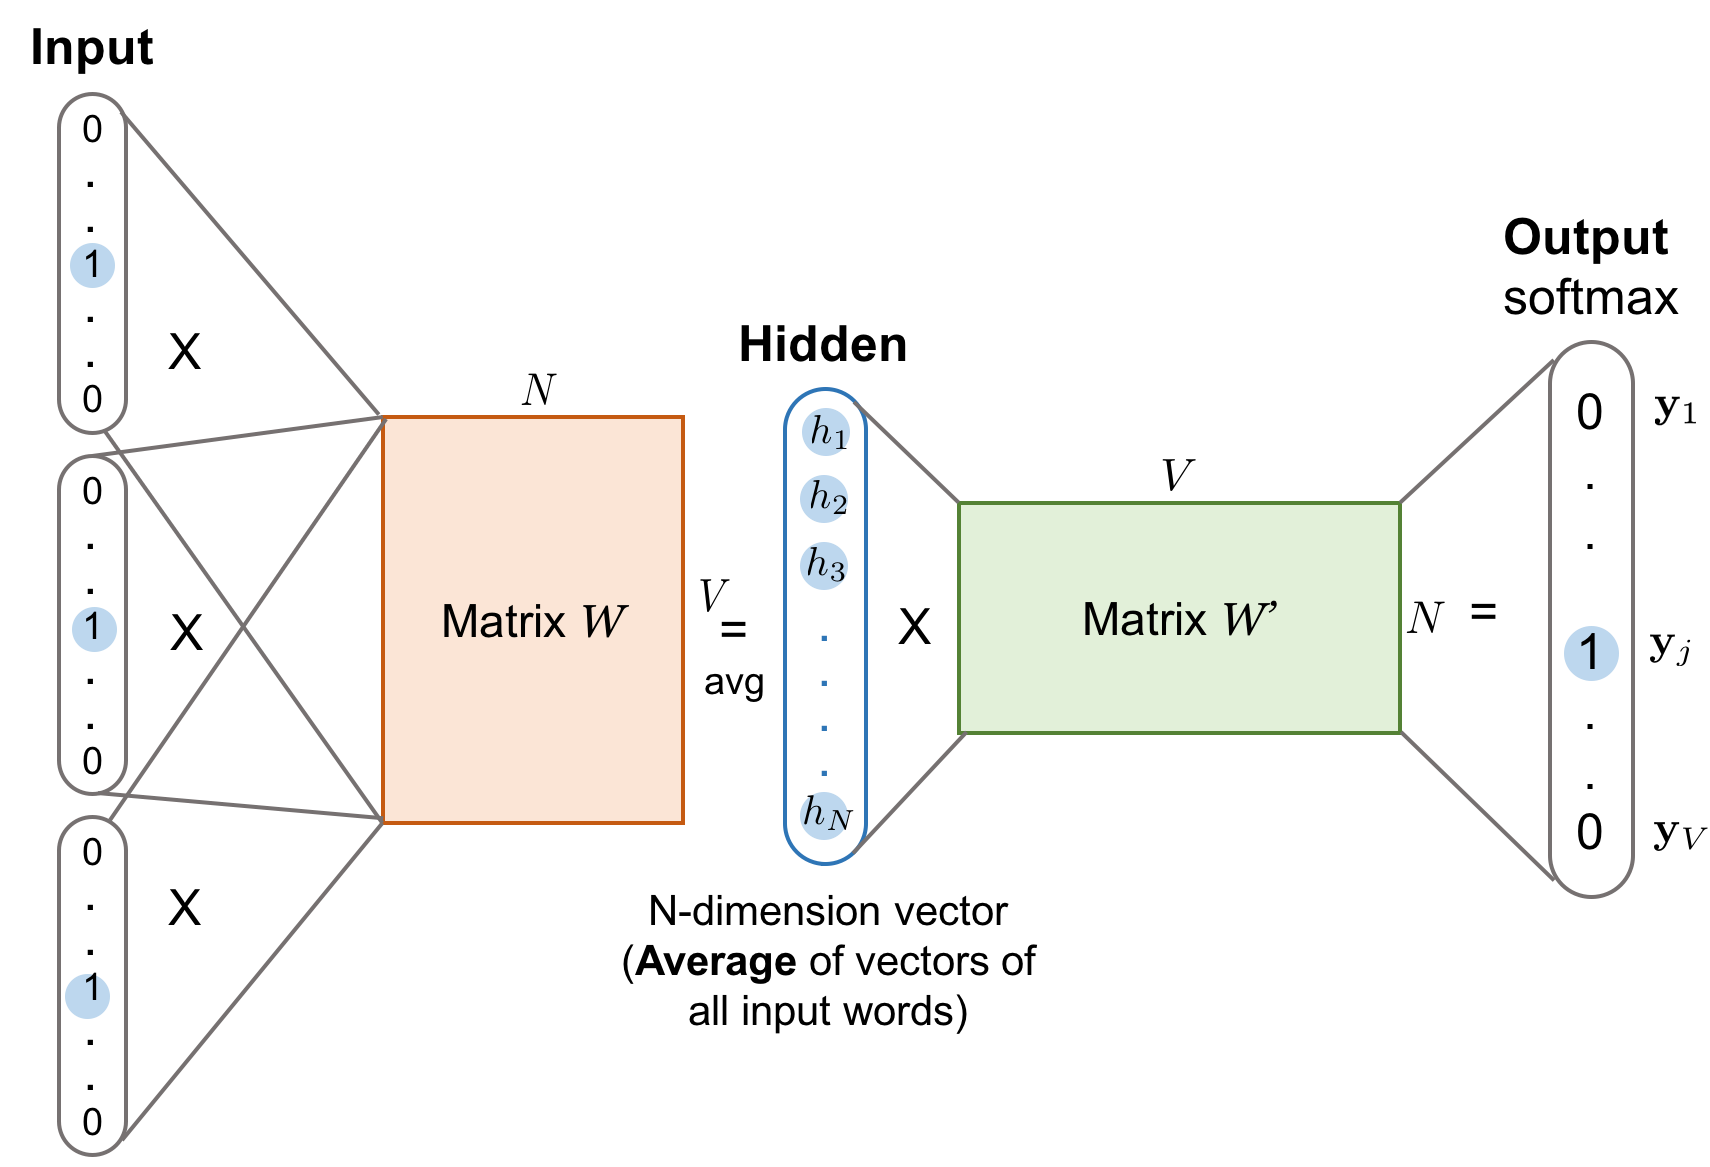
\includegraphics[width=0.8\textwidth]{word2vec-cbow.png}

iar în continuare, metoda Skip-Gram:

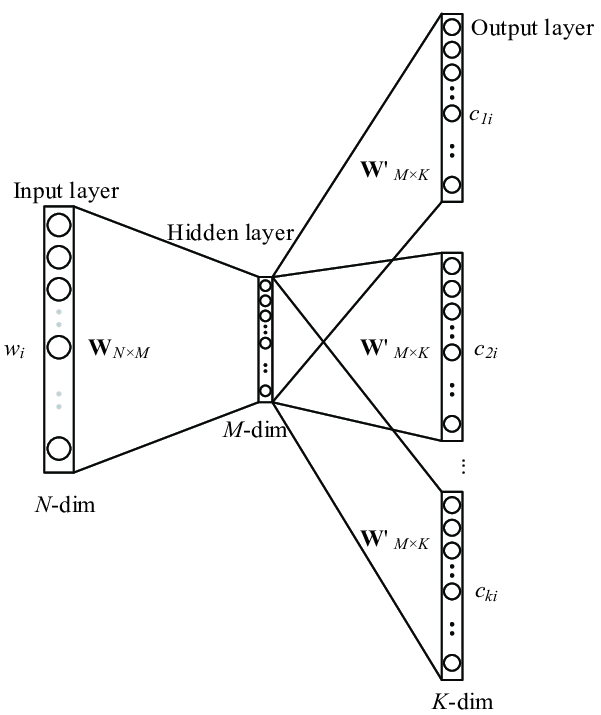
\includegraphics[width=0.8\textwidth]{skip-gram.png}



Inițial când am folosit această tehnică, am antrenat modelul Word2Vec doar cu tweet-urile din setul de antrenament,
iar acest lucru s-a dovedit destul de ineficient deoarece, după cum am specificat mai sus, setul de date este format
din tweet-uri scurte, cu multe cuvinte diferite, sub diferite forme, fapt care face și modelul Word2Vec să nu
acapareze multe cuvinte, sau să nu stabilească așa de bine vectorii cuvintelor găsite. Am avut evident rezultate 
mai bune decât în cazul n-gramelor, însă f-score-ul clasei 1 a crescut considerabil. Pentru a mări eficiența
clasificatorului final, am decis să antrenez modelul Word2Vec folosind mai multe seturi de tweet-uri, ajungând 
până la aproximativ un milion de tweet-uri. Într-adevăr s-a văzut o diferență considerabilă, f-score-ul final
pe setul de test dublându-se.

Pentru folosirea acestei metode, am utilizat librăria gensim din python, deoarece se folosește ușor. 


\section{FastText}

Metoda fasttext este o metodă ingenioasă, creată de FAIR (Facebook's AI Research Lab). Această metodă, asemănătoare
modelului Word2Vec, prin metoda CBOW sau Skip-Gram, antrenează o rețea neuronală supervizat sau nesupervizat, pentru
a descoperi caractersticle cuvintelor. Diferența de Word2Vec este faptul că nu se antrenează vectorul unui cuvânt 
în funcție de context (sau contextul în funcție de cuvânt), ci se antrenează n-gramele cuvintelor (cuvântul este împărțit în bucâți de lungime n),
după care, pentru aflarea vectorului unui cuvânt, se adună element cu element vectorii n-gramelor din care acesta este format.

Cei de la Facebook nu a făcut publice detaliile de implementare ale acestei metode, însă pune la dispoziție gratuit bibliotecile
pe care aceștia l-au creat.

Rezultatele obținute au fost puțin mai bune decât cele obținute folosind Word2Vec. Pentru partea de folosire, este evident
faptul că am folosit o bibliotecă în python, aceasta fiind fasttext.

\section{BERT}

Metoda BERT (Bidirectional Encoder Representations from Transformers), este o nouă metodă, publicată de către 
cercetători de la Google AI Language. Această inovație are ca idee de bază antrenarea bidirecțională a \href{https://www.analyticsvidhya.com/blog/2019/06/understanding-transformers-nlp-state-of-the-art-models/}{Transformatorilor}, 
în care n-o să intru în detaliu deoarece nu i-am folosit și nici nu am avut intenția. De fapt, această metodă "calculează" sensurile
cuvintelor în ambele direcții, spre deosebire de Transformatorii simpli, care o făceau ori de la dreapta la stânga, ori invers.

Această metodă a uimit prin faptul că a reușit să obțină "state of the art" (cele mai bune rezultate) în mai multe probleme
de modelare a limbajului natural. Din păcate nu am reușit să rulez această metodă, deoarece folosește prea multă memorie RAM,
dar am zis că merită menționată atât timp cât am încercat.

